\chapter{TourLive Server}
\label{sec:tourliveserver}
In den folgenden Abschnitten wird die Webapplikation TourLive Server erläutert. Dabei liegt der Fokus auf der Spezifikation und deren technischen Umsetzung. Dieses Kapitel richtet sich ins Besondere an Entwickler, welche an diesem Projekt weiterarbeiten möchten und an Personen, welche an den technischen Details interessiert sind.

\section{Software Analyse}
\subsection{Spezifikation}
Weite Teile der Anforderungen an die Webapplikation ergeben sich aus der Analyse der bestehenden Lösung. Im Einsatz ist zur Zeit eine, von der cnlab AG entwickelte \textit{\gls{php}} Webapplikation. Grundsätzlich soll die Funktionalität der bestehenden Lösung erweitert und in technologischer Sicht auf den aktuellsten Stand gebracht werden. In der folgenden Tabelle \ref{tab:tourlivewebspeztable} wird dargestellt, ob es sich um eine neue Funktion handelt oder ob eine Bestehende erweitert wurde.
\\

Die Analyse der funktionalen Anforderungen und Usecases sind im Anhang \ref{sec:tourliveusecase} umfangreich Dokumentiert.

\begin{longtable}{ p{3.5cm} | p{4.3cm} | p{4.3cm} }
	\textbf{Spezifikation} & \textbf{Altes System} & \textbf{Neues System} \\ [1ex] \hline \hline & & \\ [-1.5ex] Renn- und Etappenverwaltung & - & Benutzerfreundliche Renn- und Etappenverwaltung\\ [1ex] \hline & &  \\ [-1.5ex]
Bildübertragung & 1 Bild / Zeitpunkt (auch bei mehreren Aufnahmegeräten) & Konfigurierbare Bildübertragung\\ [1ex] \hline & &  \\ [-1.5ex]
Streckenprofil & Aktuelle Position & Alle Positionen (HTML5, SVG\footnote{HTML5 und SVG sind zwei moderne Webtechnologien um grafiken im Browser zu zeichnen})\\ [1ex] \hline & &  \\ [-1.5ex]
Zeitliche Abstände & Distanz in Zeit und km zwischen Geräten & Rückstand relativ zur Spitze in Zeit und km, sowie Durchschnittsgeschwindigkeit und Höhenmeter\\ [1ex] \hline & &  \\ [-1.5ex]
Rennsituation & Fahrer werden gruppiert dargestellt & Fahrer mit weiteren Informationen angereichert\\ [1ex] \hline & &  \\ [-1.5ex]
Rangliste & - & Aktuelle (virtuelle) Rangliste, sortierbar\\ [1ex] \hline & &  \\ [-1.5ex]
Marschtabelle & - & Marschtabelle mit Informationen und allen Positionen der Aufnahmegeräten\\ [1ex] \hline & &  \\ [-1.5ex]
Kartenausschnitt & Position der Aufnahmesysteme & Poistionen der Aufnahmesysteme (Farbe wählbar)\\ [1ex] \hline & &  \\ [-1.5ex]
Replay & Vergangene Rennen abspielbar & Rennen vor und zurück spulen nach Zeit und Renn Km\\ [1ex] \hline & &  \\ [-1.5ex]
Werbebanner & Statische Werbung & Einbetten von HTML Code für Werbeblock\\ [1ex] \hline & &  \\ [-1.5ex]
Mobile Client & - & Webseite optimiert für alle Bildschirmgrössen und Geräte\\ [1ex]  

\caption{Spezifikation TourLive Server}
\label{tab:tourlivewebspeztable}
\end{longtable}

\subsection{Evaluation Webframework}
\label{sec:tourliveserverevaluationwebframework}
Wie aus der Aufgabenstellung zu entnehmen ist, wird keine spezifische Technologie für die Umsetzung des TourLive Server festgelegt. Vielmehr ist es Teil der Arbeit eine geeignete Lösung zu evaluieren und dabei auf ein \textit{\gls{webframework}} zurückzugreifen.
Die Anforderungen an das neue TourLive System bilden die Basis für die Evaluation eines dafür geeigneten Webframeworks.
\\

In einem nächsten Schritt wurden mögliche Lösungen gesucht und auf die obigen Anforderungen geprüft. Aktuell beliebte und verbreitete Frameworks wie Django (basierend auf der Programmiersprache Python) oder Ruby on Rails seien an dieser Stelle als Beispiele erwähnt. Für die detaillierte Evaluation und Gewichtung der Kriterien wird aber auf Kapitel \ref{sec:evaluationwebframework} im Anhang verwiesen.

\subsubsection{Entscheid}
Zusammen mit dem Industriepartner fällt die Entscheidung auf das Java basierte Spring MVC Framework\footnote{Java Spring Framework Family, \url{http://springsource.org}, aufgerufen am 16.052013)}. Da die Frameworks sehr ähnliche Ideen verfolgen und sich daher, abstrakt betrachtet, kaum unterscheiden. Ausschlaggebend für diesen Entscheid waren schlussendlich die Vorkenntnisse der Studierenden in der Java Technologie. 

\subsection{Weitere Technologien}
Die folgenden weiteren Technologien wurden für die Umsetzung des TourLive Server verwendet. Im Kapitel \ref{sec:wekzeugeundentwicklungsumgebung} im Anhang sind spezifische Tools und Entwicklungsumgebungen für die weitere Entwicklung aufgeführt.

\subsubsection{ORM und Datenbank}
Für die Persistierung sämtlicher Daten wird die MySQL ähnliche, quelloffene Datenbank MariaDB\footnote{MariaDB, \url{https://mariadb.org/}, aufgerufen am 16.05.2013} verwendet. Dies ist eine Anforderung des Industriepartners cnlab AG.
\\

Die Abbildung des Models auf der Datenbank übernimmt das Java ORM Framework Hibernate\footnote{Hibernate ORM, \url{http://www.hibernate.org/}, aufgerufen am 16.05.2013}, dank unzähliger Datenbanktreiber kann ein beliebiges Datenbanksystem, unter anderem auch MariaDB, verwendet werden.

\subsubsection{Maven}
Für die Verwaltung der externen Java Libraries wird Apache Maven\footnote{Apache Maven, \url{http://maven.apache.org/}, aufgerufen am 16.05.2013} verwendet. Maven lädt die definierten Abhängigkeiten automatisch und kompiliert das Projekt. Weiter generiert Maven die Javadoc\footnote{Javadoc, \url{http://de.wikipedia.org/wiki/Javadoc}, aufgerufen am 16.05.2013} Dokumentation zum Projekt und kann Auswertungen und statische Codeanalysen erzeugen.

\subsubsection{Twitter Bootstrap}
Die Daten werden mit dem Front-End Framework Twitter Bootstap in Form einer HTML Webseite dargestellt. Twitter Bootstrap vereinfacht und beschleunigt die Entwicklung von Webseiten indem es gewisse grundlegende Elemente anbietet. Es besteht aus einer komprimierten JavaScript und einer CSS Datei und kann durch viele Plugins erweitert oder verändert werden. Twitter Bootstrap ist OpenSource und in der Entwicklergemeinde sehr beliebt, da es unter anderem Webseiten für verschiedene Bildschirmgrössen (inkl. Smartphones und Tablets) optimal anpasst.

\subsection{Domain Model}
In der folgenden Abbildung \ref{fig:tourliveserverdomainmodel} wird die Problem Domain schematisch dargestellt. Die Renn- und insbesondere die Etappenklasse stehen im Zentrum der Abbildung, da die Informationen dort zusammengeführt werden. Darauf folgt die Umsetzung der einzelnen Elementen im Abschnitt \ref{sec:tourliveserversoftwaredesign}. 

\begin{figure}[H]
	\centering
	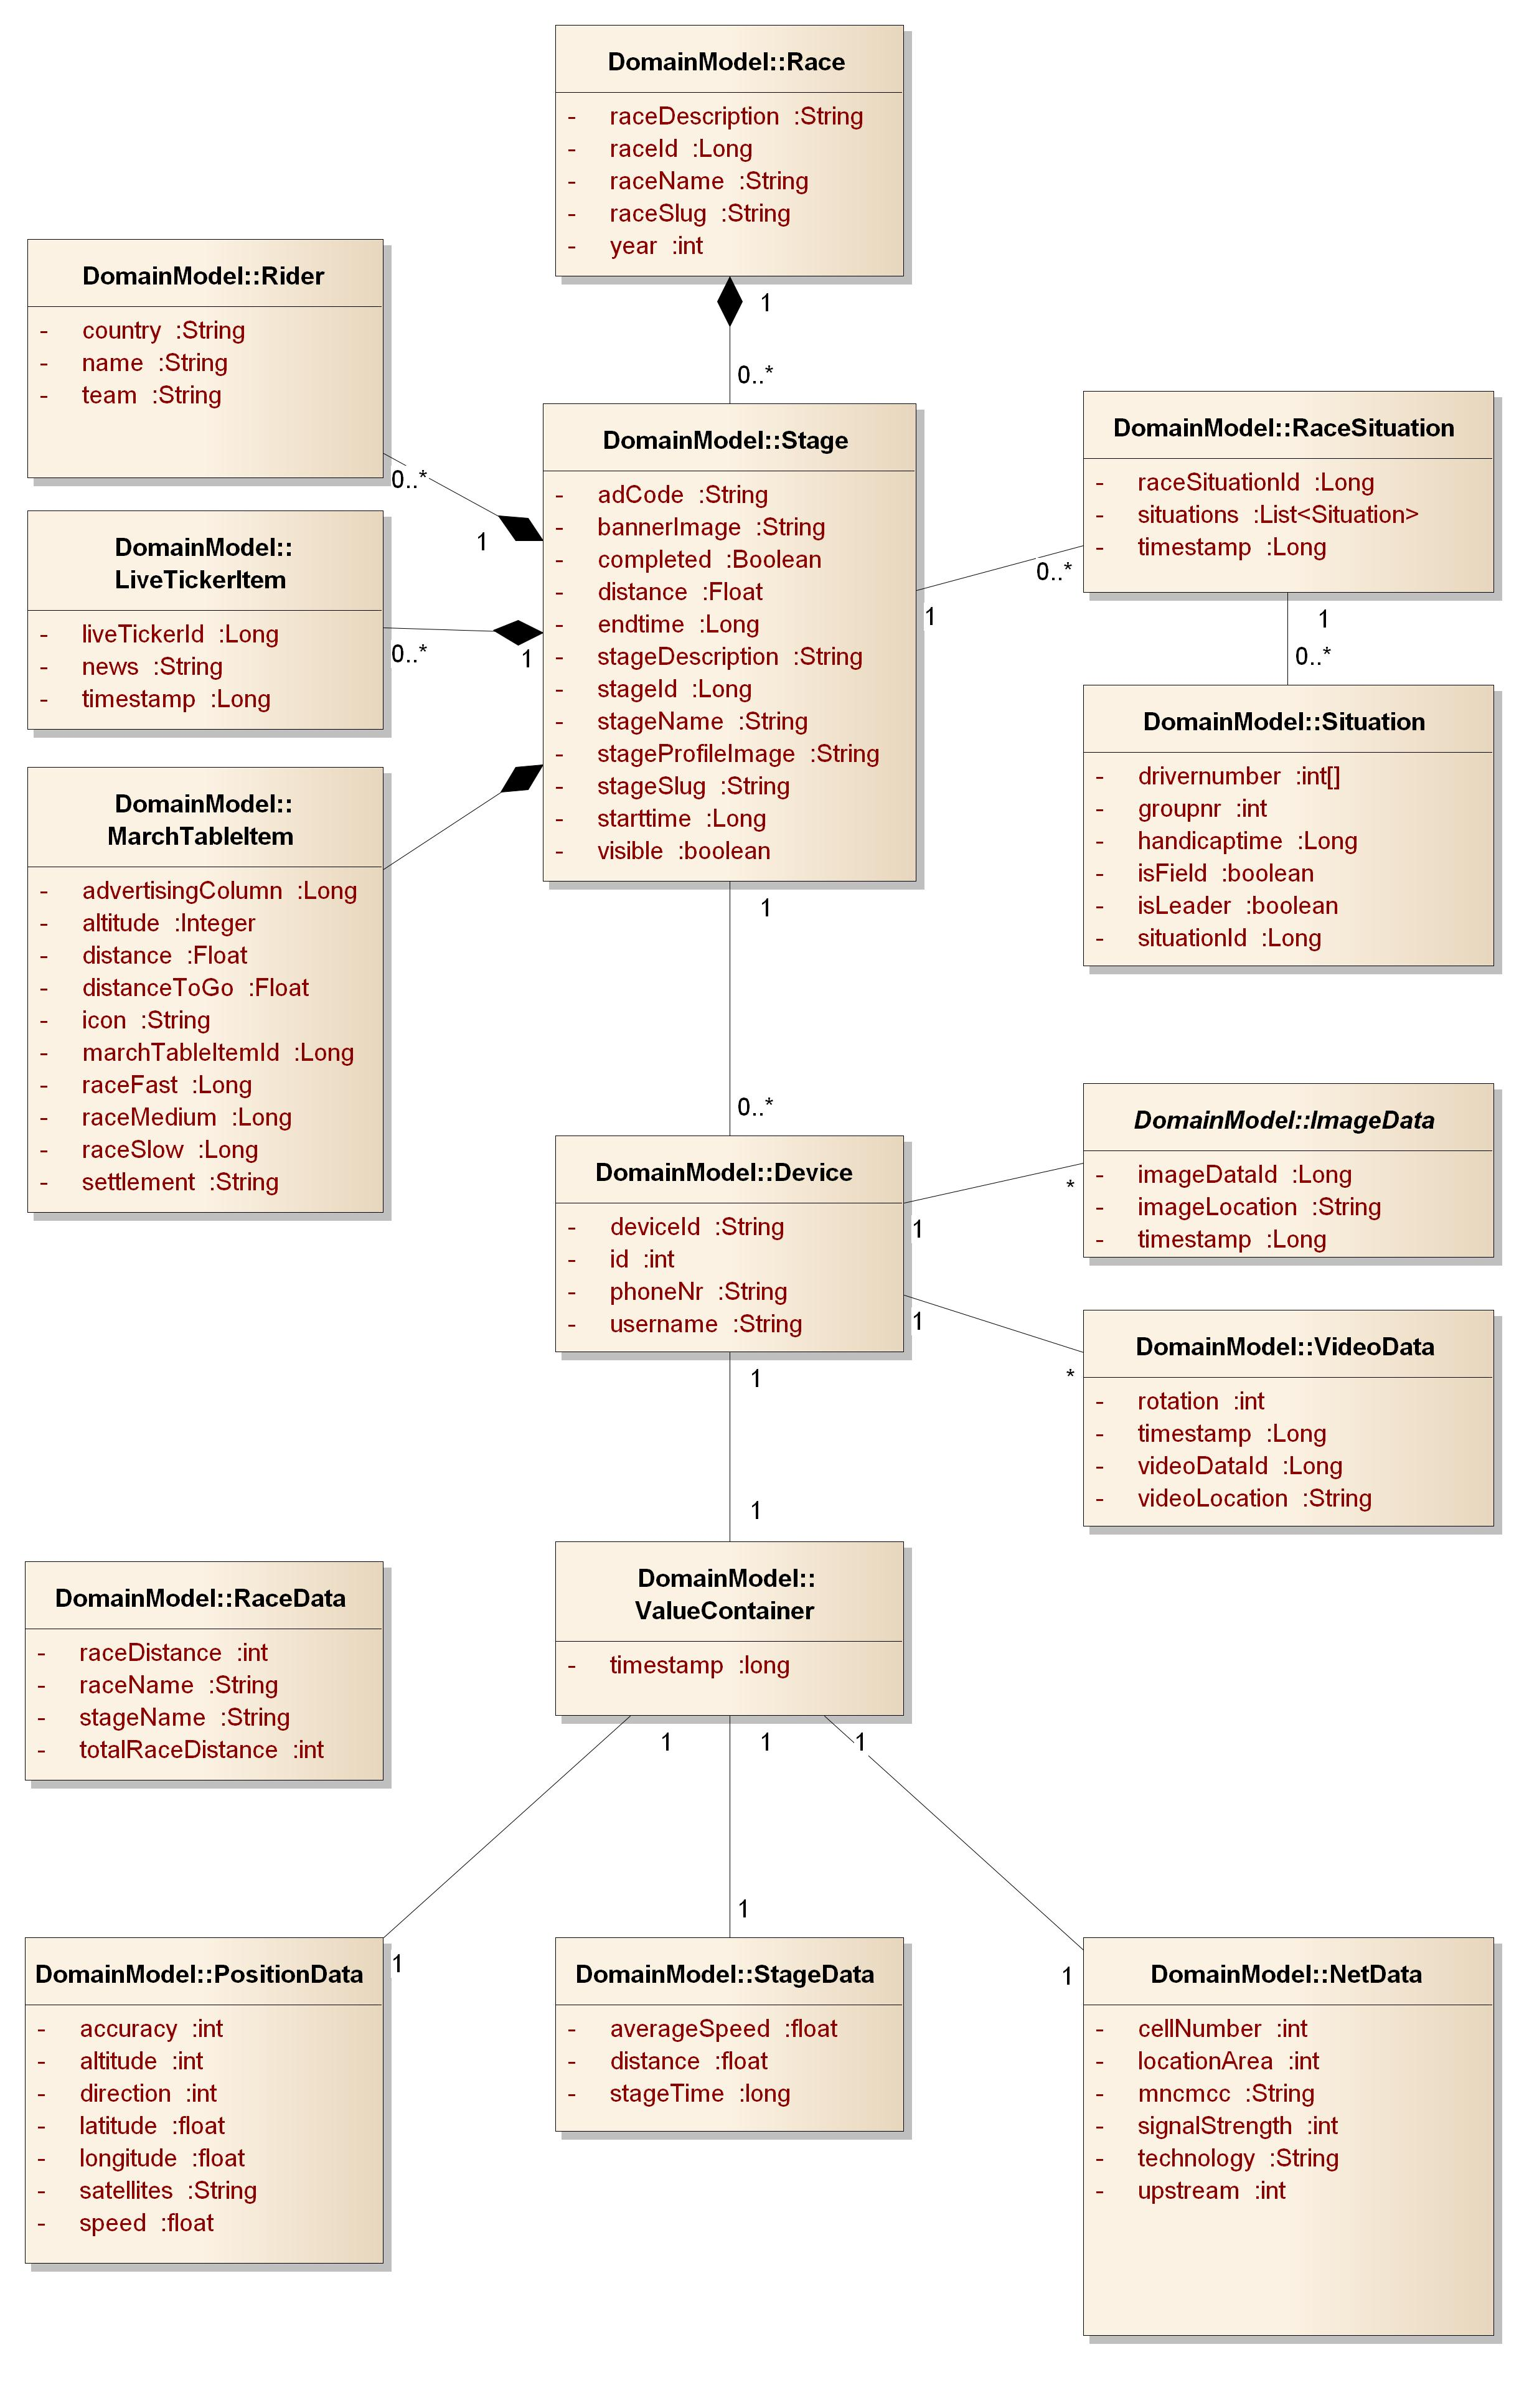
\includegraphics[width=130mm]{images/tourliveweb/TourLiveServer_DomainModel_ohneRand.jpg}
	\caption{Domain Model des TourLive Servers}
	\label{fig:tourliveserverdomainmodel}
\end{figure}
\newpage

\section{Software Design}
\label{sec:tourliveserversoftwaredesign}
Dieser Abschnitt behandelt die Umsetzung der Spezifikationen zum Endzustand. Nach einer kurzen Architekturübersicht wird jede Teilkomponente einzeln erläutert.

\subsection{Architektur und Übersicht}
Der TourLive Server übernimmt zwei grundsätzlich Funktionen, zum einen die Präsentation der Daten und zum anderen die Schnittstelle (\textit{\gls{api}}) für die Aufnahmegeräte und Drittentwickler.
\begin{figure}[H]
	\centering
	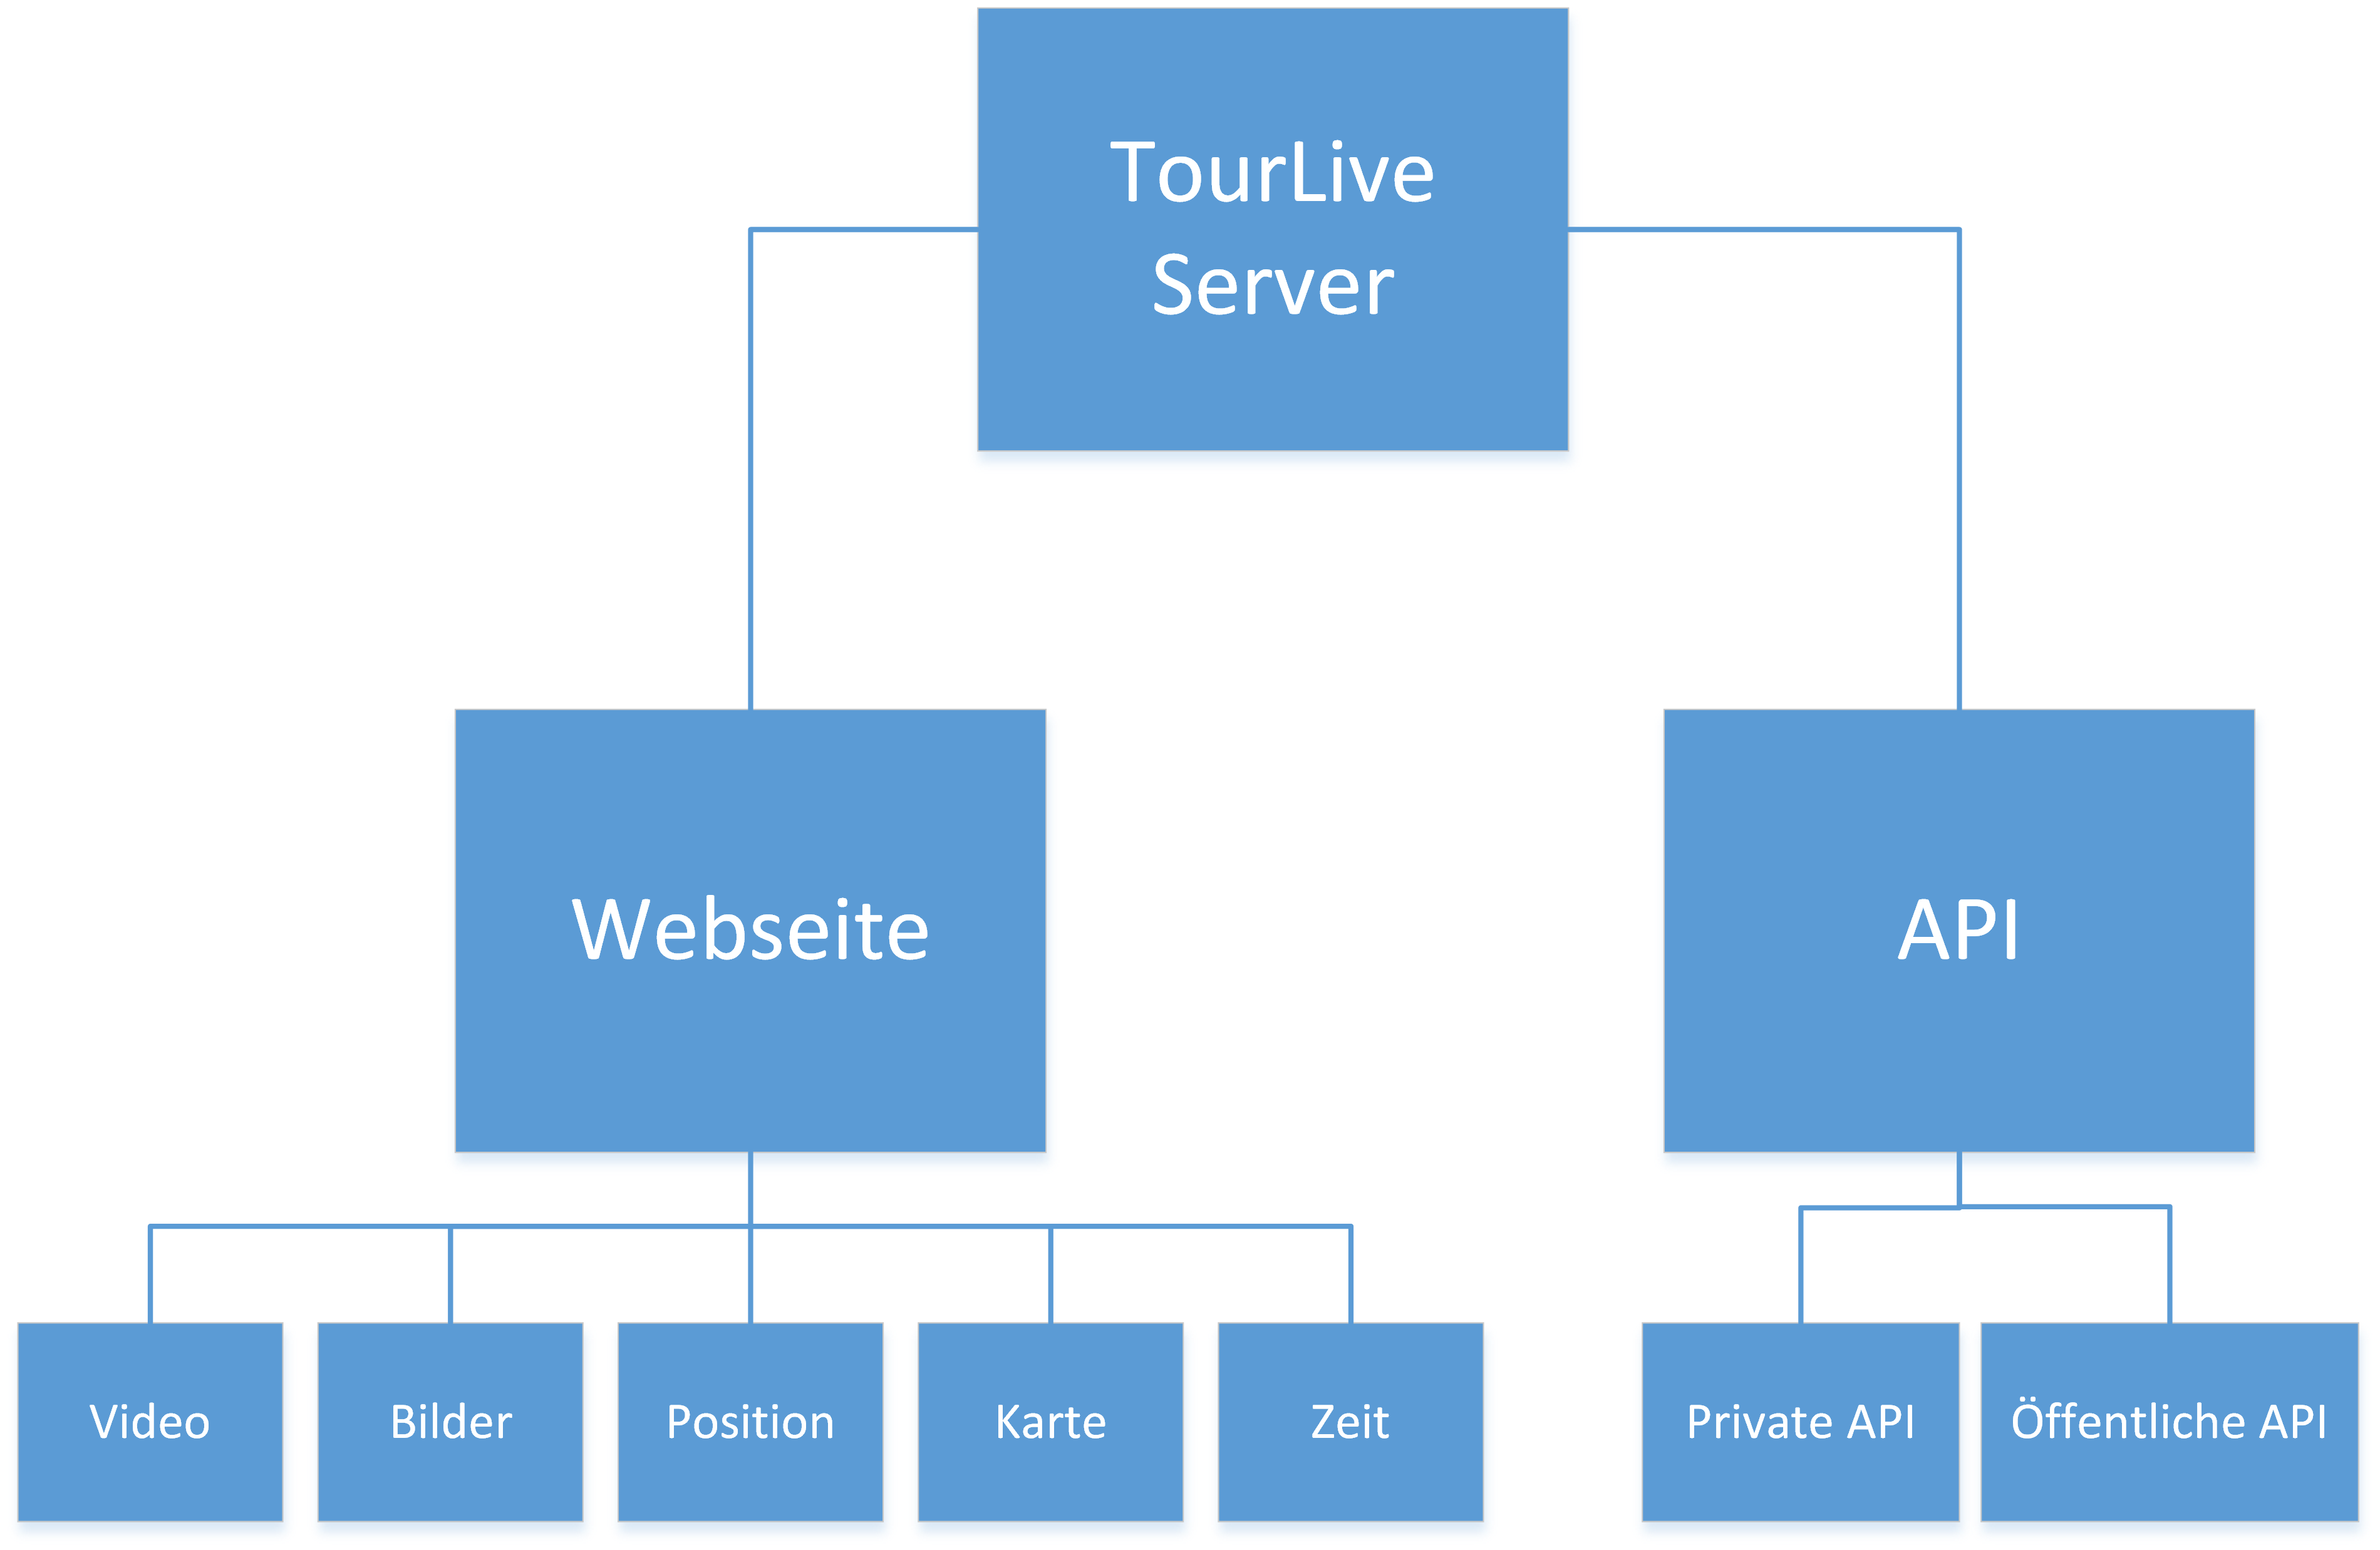
\includegraphics[width=130mm]{images/tourliveweb/uebersicht_tourlive.png}
	\caption{Grobstruktur des TourLive Servers}
	\label{fig:grobstrukturtourliveserver}
\end{figure}
Diese Aufteilung wurde bewusst so gewählt, da es die Möglichkeit offen lässt, die Dienste auf mehrere Server aufzuteilen. Aus dem Requirements Engineering kam hervor, dass das System auch unter grosser Last für die Datenerfassung immer zur Verfügung stehen muss. In der Entwicklungsphase wurde darauf verzichtet das System auf mehrere Server aufzuteilen, da es das Testing erschwert.

\subsection{Schichtenmodell und Packagediagramm}
Ein Spring MVC Projekt legt eine gewisse Struktur vor, wie eine Webapplikation aufgebaut werden soll. Dadurch fördern sie gute Programmierpraktiken und erzeugen gewisse Standards. Auch beim TourLive Server wurden diese Vorgaben angewendet.
\\

\begin{figure}[H]
	\centering
	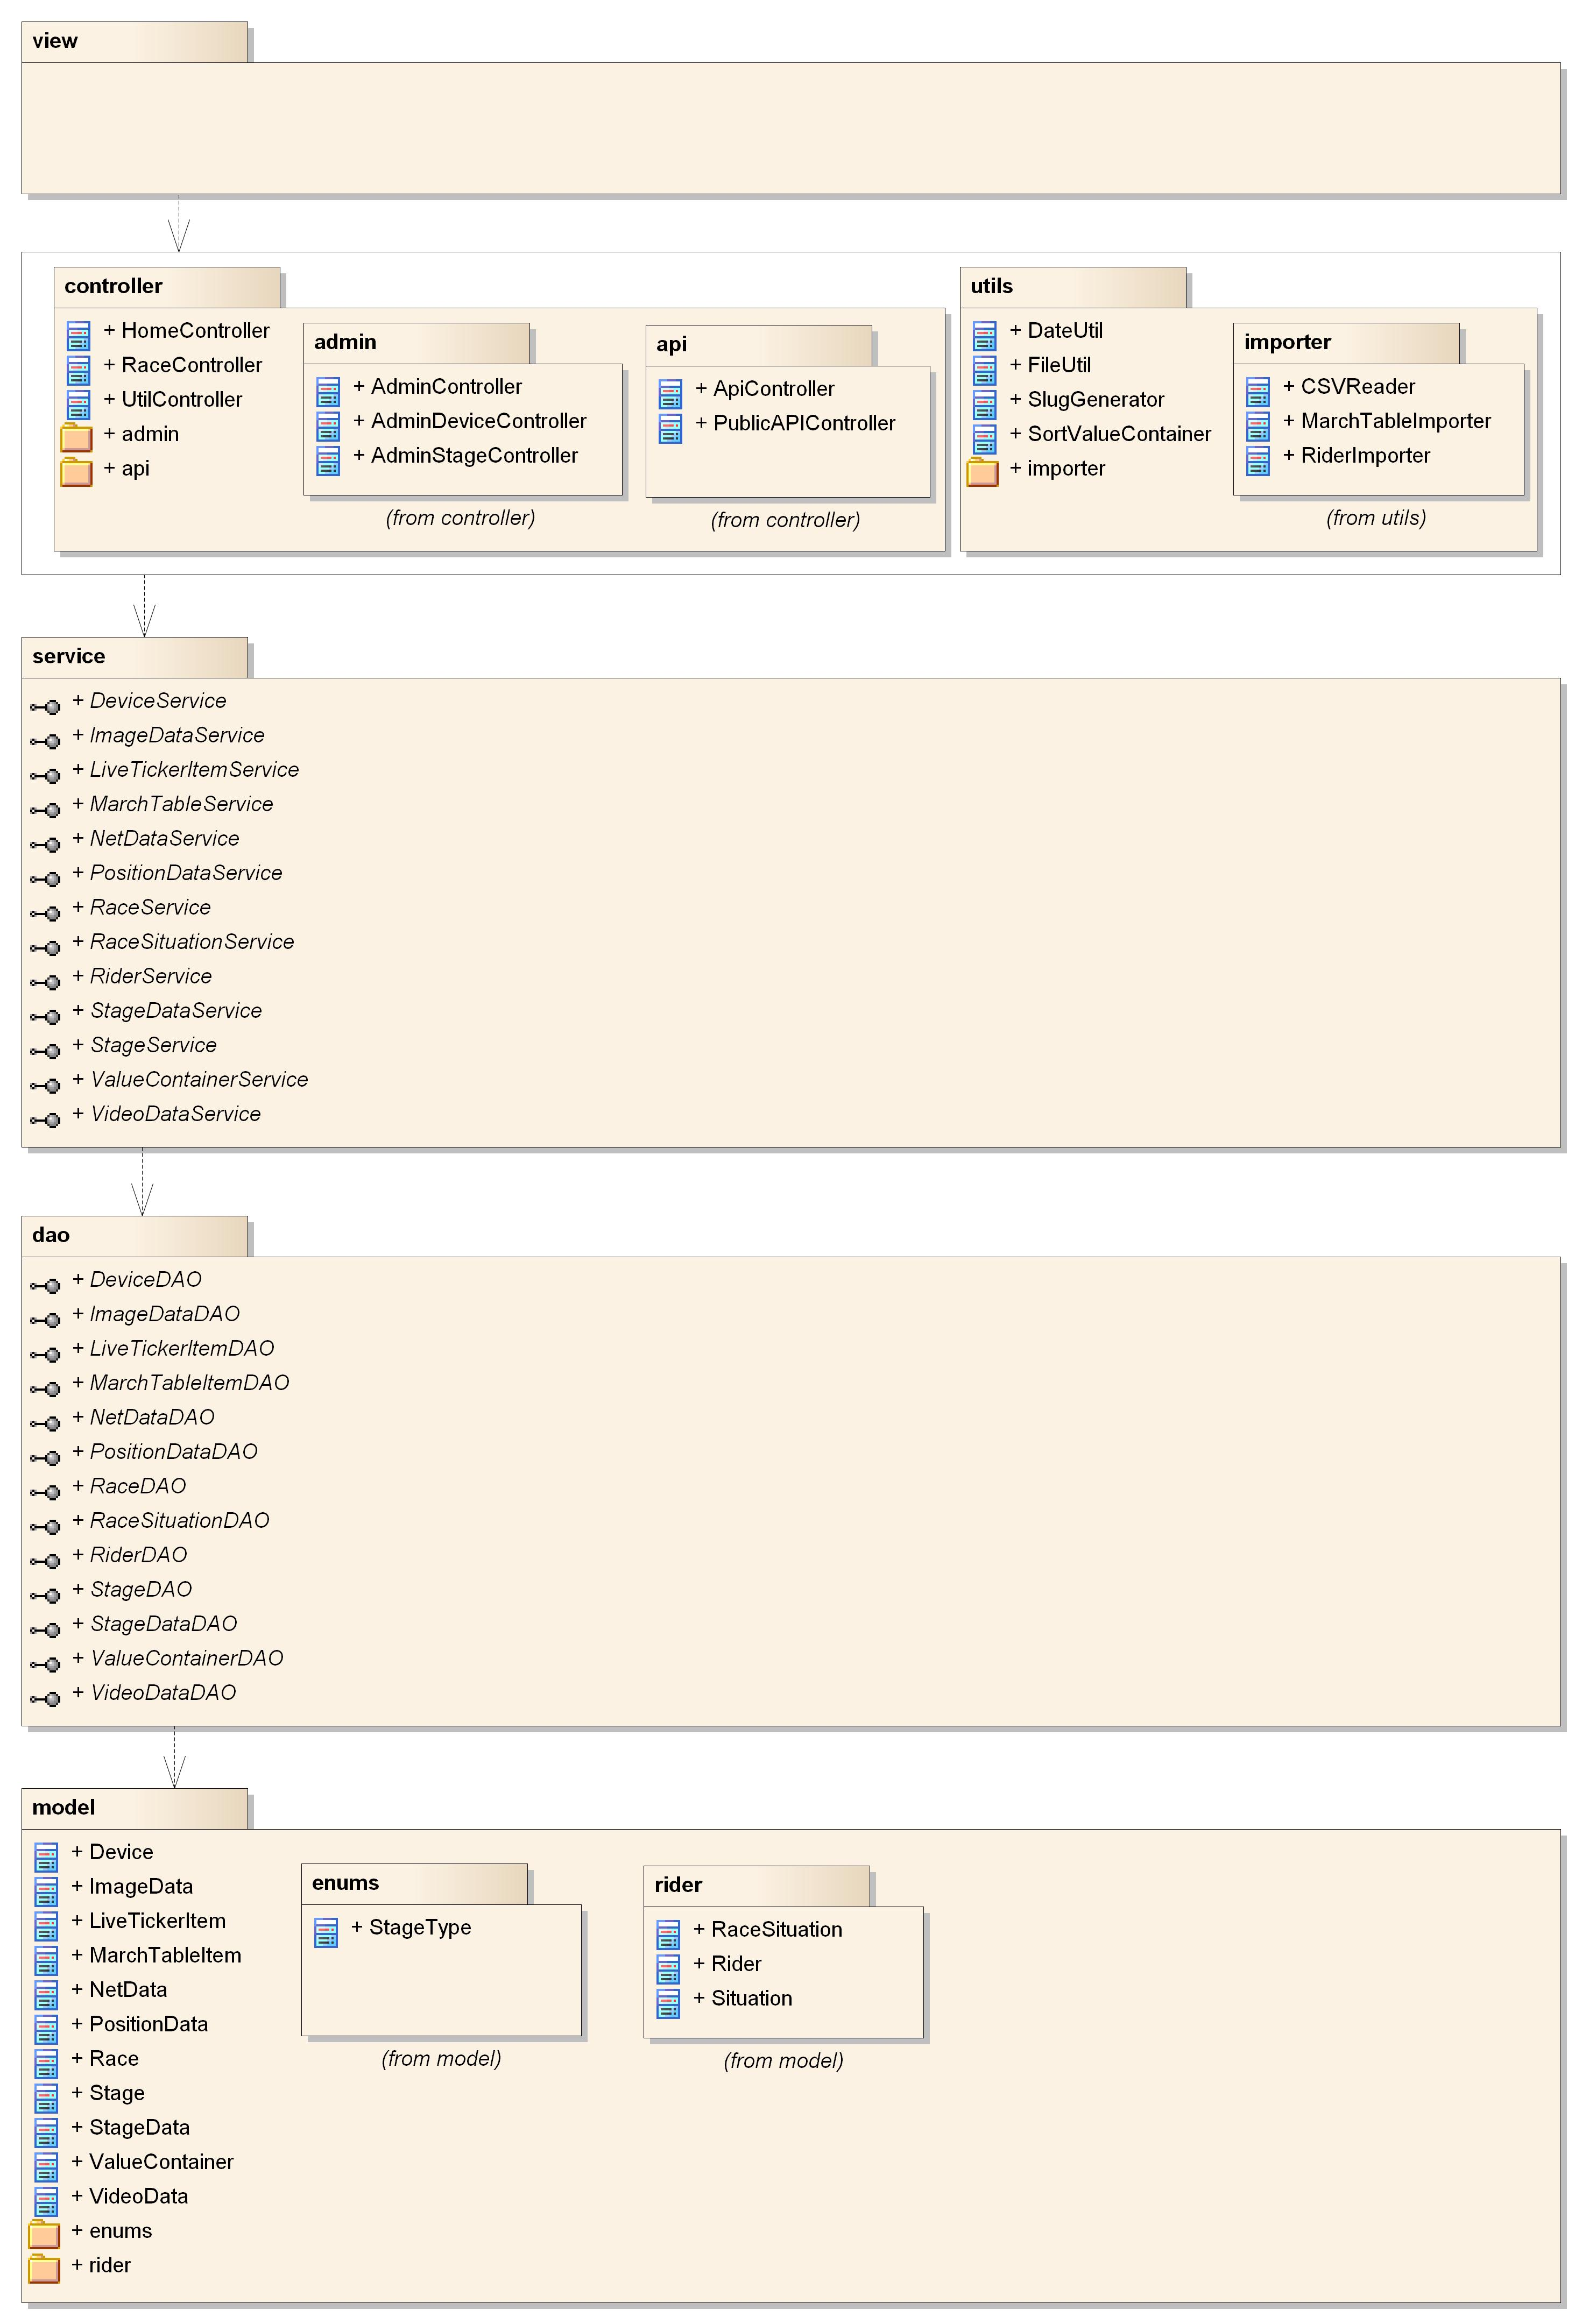
\includegraphics[width=130mm]{images/tourliveweb/TourLiveServer_Package_ohneRand.jpg}
	\caption{Packagediagramm des TourLive Servers}
\end{figure}\label{fig:tourlivewebpackage}

Im Packagediagramm \ref{fig:tourlivewebpackage} sind die Schichten der Applikation zu erkennen. So wurde das Domainmodel im Package \textit{Model} abgebildet, die Datenzugriffsobjekte im \textit{DAO} Package und die dazugehörige Service Schicht im Package \textit{Service}. Die Anfragen werden durch die Zugriffscontroller im Package \textit{Controller} bearbeitet. Um wiederkehrende Tasks zu zentralisieren, wurden diese im Package \textit{Utils} zusammengefasst, so z.B. das Formatieren Zeiten und Daten.

\subsection{Video}
Eine Anforderung war es, eine Lösung zu erarbeiten, welche es ermöglicht mit den Aufnahmegeräten Video Streams aufzuzeichnen und an den Server zu übermitteln. Dazu gibt es verschiedene Ansätze mit entsprechenden Vor- und Nachteilen. Im TourLive System im Einsatz ist eine eigene Entwicklung welche genau auf die Bedürfnisse angepasst ist. Die Geräte nehmen Videosequenzen auf und übertragen diese an den Server. Der Server konvertiert diese Sequenzen vom mp4 in das ogg Format. Dazu wird die externe Library Xuggler\footnote{Xuggler, \url{http://www.xuggle.com/xuggler}, aufgerufen am 04.06.2013} verwendet. Mit diesem Schritt sind die Browser Google Chrome, Mozilla Firefox und Microsoft Internet Explorer fähig die Videosequenzen abzuspielen. Zusätzlich wird ein VideoData Objekt (vgl. Abbildung \ref{fig:tourliveserverdomainmodel}) in der Datenbank angelegt, welches den Aufnahmezeitpunkt und die Geräte ID, eine allfällige Rotation, sowie den Pfad zur Videodatei enthält. Wenn nun ein Gerät einer Etappe zugewiesen ist und Videosequenzen vorhanden sind, wird die aktuellste Sequenz ausgeliefert. Der Videoplayer meldet wenn die Videosequenz beendet ist und lädt, falls möglich, die nächste Sequenz via AJAX automatisch nach, dies wird im Quellcode \ref{code:ajaxquellcode} dargestellt. Falls kein neues Video verfügbar ist, wird nach 8 Sekunden erneut versucht ein Video zu laden. Dadurch wird auch bei einem temporären Ausfall der Aufnahmegeräte die Videowiedergabe fortgesetzt, sobald diese wieder verfügbar ist.

\begin{lstlisting}[language=JavaScript, caption=Automatisches Nachladen von Videosequenzen, label=code:ajaxquellcode]
var videoPlayer1 = document.getElementById('video1');
videoPlayer1.addEventListener('ended', function(){
	loadNext(videoPlayer1);
});

function loadNext(videoPlayer){
	$.ajax({
		type : "POST",
		dataType: "json",
		url : "/meineetappe/nextvideo",
		data : {
			deviceId : 'meinedeviceid',
			afterId: videoPlayer.id,
		},
		success : function(data) {
			if (data){
				$('#mp4').attr('src', 'http://media.tourlive.ch/'+ data.videoLocation + '.mp4');
				$('#ogg').attr('src', 'http://media.tourlive.ch/'+ data.videoLocation + '.ogg');
				videoPlayer.id= "video" + data.videoDataId;
				videoPlayer.load();
			} else {
			// try again in 8s
				window.setTimeout(function(){loadNext(videoPlayer)},8000);
			}
		}
	});
\end{lstlisting}

\subsection{Bilder}
Die Aufnahme der Bilder funktioniert nach einem ähnlichen Muster. Die aufgezeichneten Bilder werden auf dem Server abgelegt und ein ImageData Objekt in der Datenbank erzeugt. Im ImageData Objekt wird, wie schon beim Video, der Aufnahmezeitpunkt, die Geräte ID sowie der Bildpfad gespeichert. Wie in Abbildung \ref{fig:bildaufzeichnung} zu sehen ist, wird beim Aufruf einer Seite das aktuellste verfügbare Bild pro Gerät angezeigt und mit dem Aufnahmezeitpunkt beschrieben.
\begin{figure}[H]
	\centering
	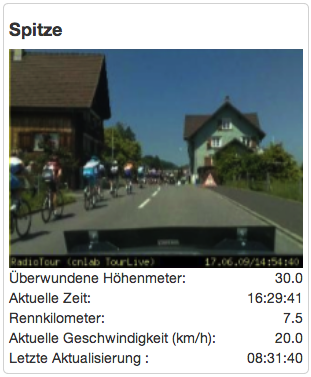
\includegraphics[width=70mm]{images/tourliveweb/bildaufzeichnung.png}
	\caption{Aufgezeichnetes Bild mit Informationen ergänzt}
	\label{fig:bildaufzeichnung}
\end{figure}

\subsection{Positionsdaten}
Die Positionsdaten werden in Form eines ValueContainers gespeichert und übertragen. Ein beispielhafter ValueContainer ist im Folgenden in der \textit{\gls{json}} Notation dargestellt.

\begin{figure}[H]
	\centering
	\lstinputlisting[language=json]{jsonfiles/valuecontainer.json}
	\caption{Beipsiel ValueContainer in der JSON Notation}
	\label{fig:valuecontainerjson}	
\end{figure}

Der Container setzt sich aus den drei Objekten \textit{netData}, \textit{positionData} und \textit{stageData} zusammen, hinzu kommt zu jedem Container das Device Objekt sowie der aktuelle Zeitpunkt als Timestamp. Daher auch der Name ValueContainer, weil darin verschiedene Daten gesammelt und übermittelt werden.
\\

Die ValueContainer bilden das Herz der Informationsquelle. Alleine durch sortieren nach dem Feld \textit{distance} im Objekt \textit{stageData} wird festgestellt, welches Gerät an der Spitze mitfährt und wie viel Prozent der Gesamtstrecke zurückgelegt wurde. Da die ValueContainer nicht einer Etappe sondern einem Gerät zugeordnet sind, können auch nachträglich noch Geräte einer Etappe hinzugefügt oder entfernt werden. Um die Positionsdaten für eine Etappe zu erhalten werden alle ValueContainer vom Startzeitpunkt bis zum Endzeitpunkt einer Etappe gefiltert und alle mit der Geräte ID eines Gerätes welches der Etappe zugeordnet ist ausgewählt. Um ein vergangenes Rennen wieder abzuspielen wird die zeitliche Grenze welche durch die Etappenendzeit gegeben war, durch einen beliebigen Zeitpunkt ( > Startzeit) ersetzt. Dadurch werden immer nur diejenigen Container ausgewählt, welche bis zum angezeigten Zeitpunkt aufgezeichnet wurden.
\\

Um die Daten zu visualisieren werden verschiedene Elemente verwendet. Der geografische Verlauf der Strecke wird auf einer Karte eingezeichnet. Jedes Aufnahmegeräte (\textit{device}) hat zusätzlich ein Feld \textit{color}, welches die Farbe auf der Karte bestimmt.
\begin{figure}[H]
	\centering
	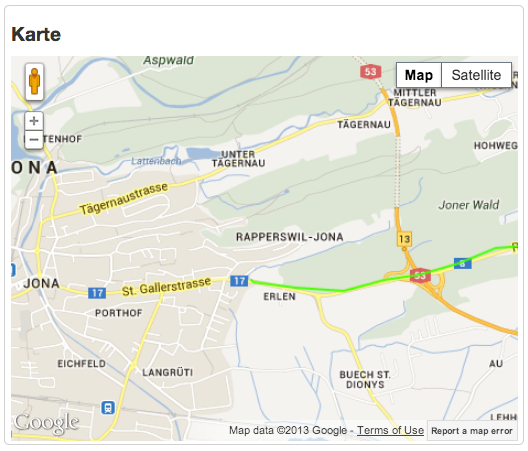
\includegraphics[width=110mm]{images/tourliveweb/karte_neu.png}
	\caption{Kartenausschnitt mit zurückgelegter Strecke eines Gerätes}
\end{figure}

Ein Aufnahmegerät fährt in der Regel an der Spitz mit, ein zweites hinter dem Feld. Die Spitze setzt sich im Laufe des Rennens ab und der Abstand wird grösser. Die Entwicklung dieses Abstands ist für Radsportbegeisterte sehr spannend zu beobachten. Diese Berechnung wird ebenfalls durch die ValueContainers ermöglicht. Sobald mehr als ein Gerät einer Etappe zugeordnet ist, beginnt die Berechnung des Abstandes nach dem folgenden Algorithmus.
\begin{quotation}
\textit{Für jeden ValueContainer in einer Etappe mache folgendes:
Suche pro Gerät den ValueContainer welcher die nächsttiefere Etappendistanz im Vergleich zum obigen Container aufweist, falls dieser Distanzunterschied kleiner als eine definierte Grösse ist (Standardwert 500m) so wähle den Container mit der kleinsten Zeit. Vergleiche diese Zeit mit dem ursprünglichen Container, ist die Zeit des ursprünglichen Containers grösser, so ist die Differenz der Zeiten den Rückstand für diesen Container, andernfalls ist der ursprüngliche Container zu dem Zeitpunkt an der Spitze}
\end{quotation}

Diese Berechnung ist sehr Aufwändig und wird mit steigender Anzahl ValueContainers immer langsamer. Im lokalen Testumfeld mit weniger als 1000 ValueContainer wird diese Berechnung kaum bemerkt. Beim ersten Testlauf stellte sich jedoch heraus, dass diese Werte zwischengespeichert werden müssen, da die Liveberechnung zu lange dauern würde. Bei jedem Seitenaufruf werden nur die neu hinzugekommenen ValueContainer berechnet, dadurch wird das System schneller, je mehr Benutzer auf der Seite sind, da die Anzahl neu zu berechnender Werte immer kleiner wird. Im Administrationsbereich kann die manuelle Berechnung aller ValueContainer neu gestartet werden. Dieser Vorgang ist notwendig, wenn nachträglich ein weiteres Gerät zur Etappe hinzugefügt wird.
\\

Sämtliche Rückstände werden in einer Grafik (vgl. Abbildung  \ref{fig:abstandsentwicklung2}) dargestellt. In der X-Achse sind die zurückgelegten Rennkilometer und in der Y-Achse die Rückstände in Sekunden. Für das Aufnahmegerät an der Spitze ist diese Kurve komplett flach, daher wird diese weggelassen.

\begin{figure}[H]
	\centering
	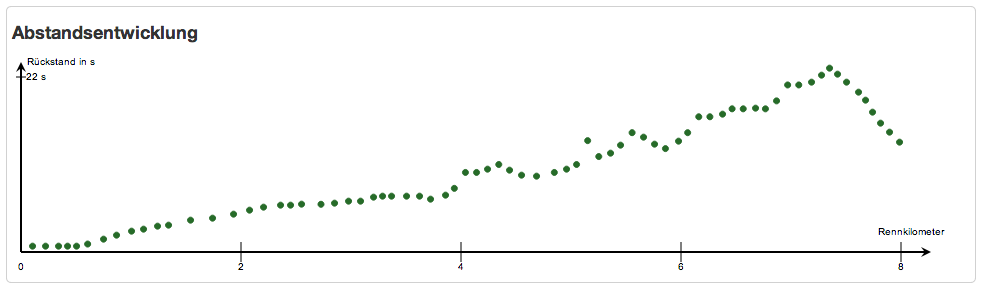
\includegraphics[width=130mm]{images/tourliveweb/abstandsentwicklung2.png}
	\caption{Abstandsentwicklung am Ende eines fiktiven Rennens}
	\label{fig:abstandsentwicklung2}
\end{figure}

\subsection{Interne API}
Mit der internen \gls{api} wird die Schnittstelle zwischen den Aufnahmesystemen und dem TourLive Server bezeichnet. Diese Schnittstelle wird genauer im Kapitel \ref{sec:tourliveserverapi} erklärt.

\subsection{Public API}
Für die aufgezeichneten Daten wurde ebenfalls eine öffentliche Schnittstelle erstellt. Drittentwicklern wird es ermöglicht die Positionsdaten in ihren Anwendungen zu verwenden und die Bilder als auch die Videosequenzen abzurufen. Die Schnittstelle ist zum jetzigen Zeitpunkt uneingeschränkt nutzbar. Für den produktiven Betrieb von TourLive wäre eine Authentifizierung für die Benutzung der Schnittstelle wünschenswert, eine solche ist aber nicht Teil dieser Arbeit. Die öffentliche Schnittstelle wird im Kapitel \ref{sec:tourlivepublicapi} detailliert erläutert.

\subsection{XML basierte Konfiguration}
Die Konfiguration in Spring geschieht einerseits über Java Annotationen wie sie beim TourLive Server z.B. bei den Controllern zum Einsatz kommen, andererseits werden Servlet und Datenbankeinstellungen sowie sämtliche Abhängigkeiten zu anderen Libraries in XML Dateien konfiguriert. Die wichtigsten Dateien werden im folgenden aufgezeigt.

\subsubsection{web.xml}
Im web.xml wird zugewiesen, welches Servlet welche Ressource ansteuert. Weiter werden die Filter definiert, welche angewendet werden sollen. Filter erlauben es Anfragen vor oder nach zu bearbeiten. Im TourLive Server werden zwei Filter verwendet, der Sitemesh Filter welcher wiederverwendbare Elemente (z.B. Menu oder Footer) in den JSP Seiten auslagert. Der zweite Filter schützt den Administrationsbereich vor nicht authentifiziertem Zugriff. Bei diesem Security Filter kann eine Ressource komplett geschützt werden. Die weitere Konfiguration findet in der security.xml Datei statt.

\subsubsection{tourlive-servlet.xml}
Damit die von den Controllern erstellten Models auch auf den JSP Seiten abgebildet werden können wird ein ViewResolver verwendet. In der XML Datei wird zusätzlich angegeben wo sich die JSP Seiten befinden. Weiter werden die Internationalisierung und die Auslieferung von statischen Ressourcen, wie Bilder und StyleSheets, definiert.

\subsubsection{hibernate.xml}
Das Datenbankmapping geschieht mit Hibernate. In der hibernate.xml Datei werden die Datenbankeinstellungen vorgenommen. Zusätzlich wird hier die SessionBean deklariert, damit werden die Abfragen auf der Datenbank letztendlich ausgeführt.

\subsubsection{root-context.xml}
Im Root Context wird definiert, dass die weitere Konfiguration durch Java Annotationen interpretiert werden soll. Weiter werden die Konfigurationen der Datenbank sowie umgebungsspezifische Einstellungen importiert. Das Pendant zum Root Context für die Testumgebung ist der Test Context.

\subsubsection{security.xml}
Die Sicherheitsparameter, welche von Spring geladen werden, sind in der security.xml Datei definiert. So kann eine Login- und eine Logout-Seite angegeben werden. An dieser Stelle wird auch definiert, dass sämtliche Zugriffe auf die Administrationsseiten nur nach Authentifizierung stattfinden können.
\\

Die TourLive Server Anwendung verfügt nur über zwei Benutzergruppen, nicht authentifizierte Besucher und Administratoren. Daher wurde auf eine aufwändige Benutzerverwaltung verzichtet und nur ein Administrationsbenutzer fest in der XML Datei definiert.

\section{Realisierung}
Der für die Öffentlichkeit sichtbare Teil dieser Arbeit besteht aus den aufbereiteten Daten. Auf der Startseite wird jeweils die aktuellste Etappe angezeigt alle anderen Rennen können über die Navigation im Kopfbereich erreicht werden. In der Abbildung \ref{fig:tourlivewebansicht} ist ein fiktives Beispiel der ersten Etappe der Tour de Suisse 2013 dargestellt.

\begin{figure}[H]
	\centering
	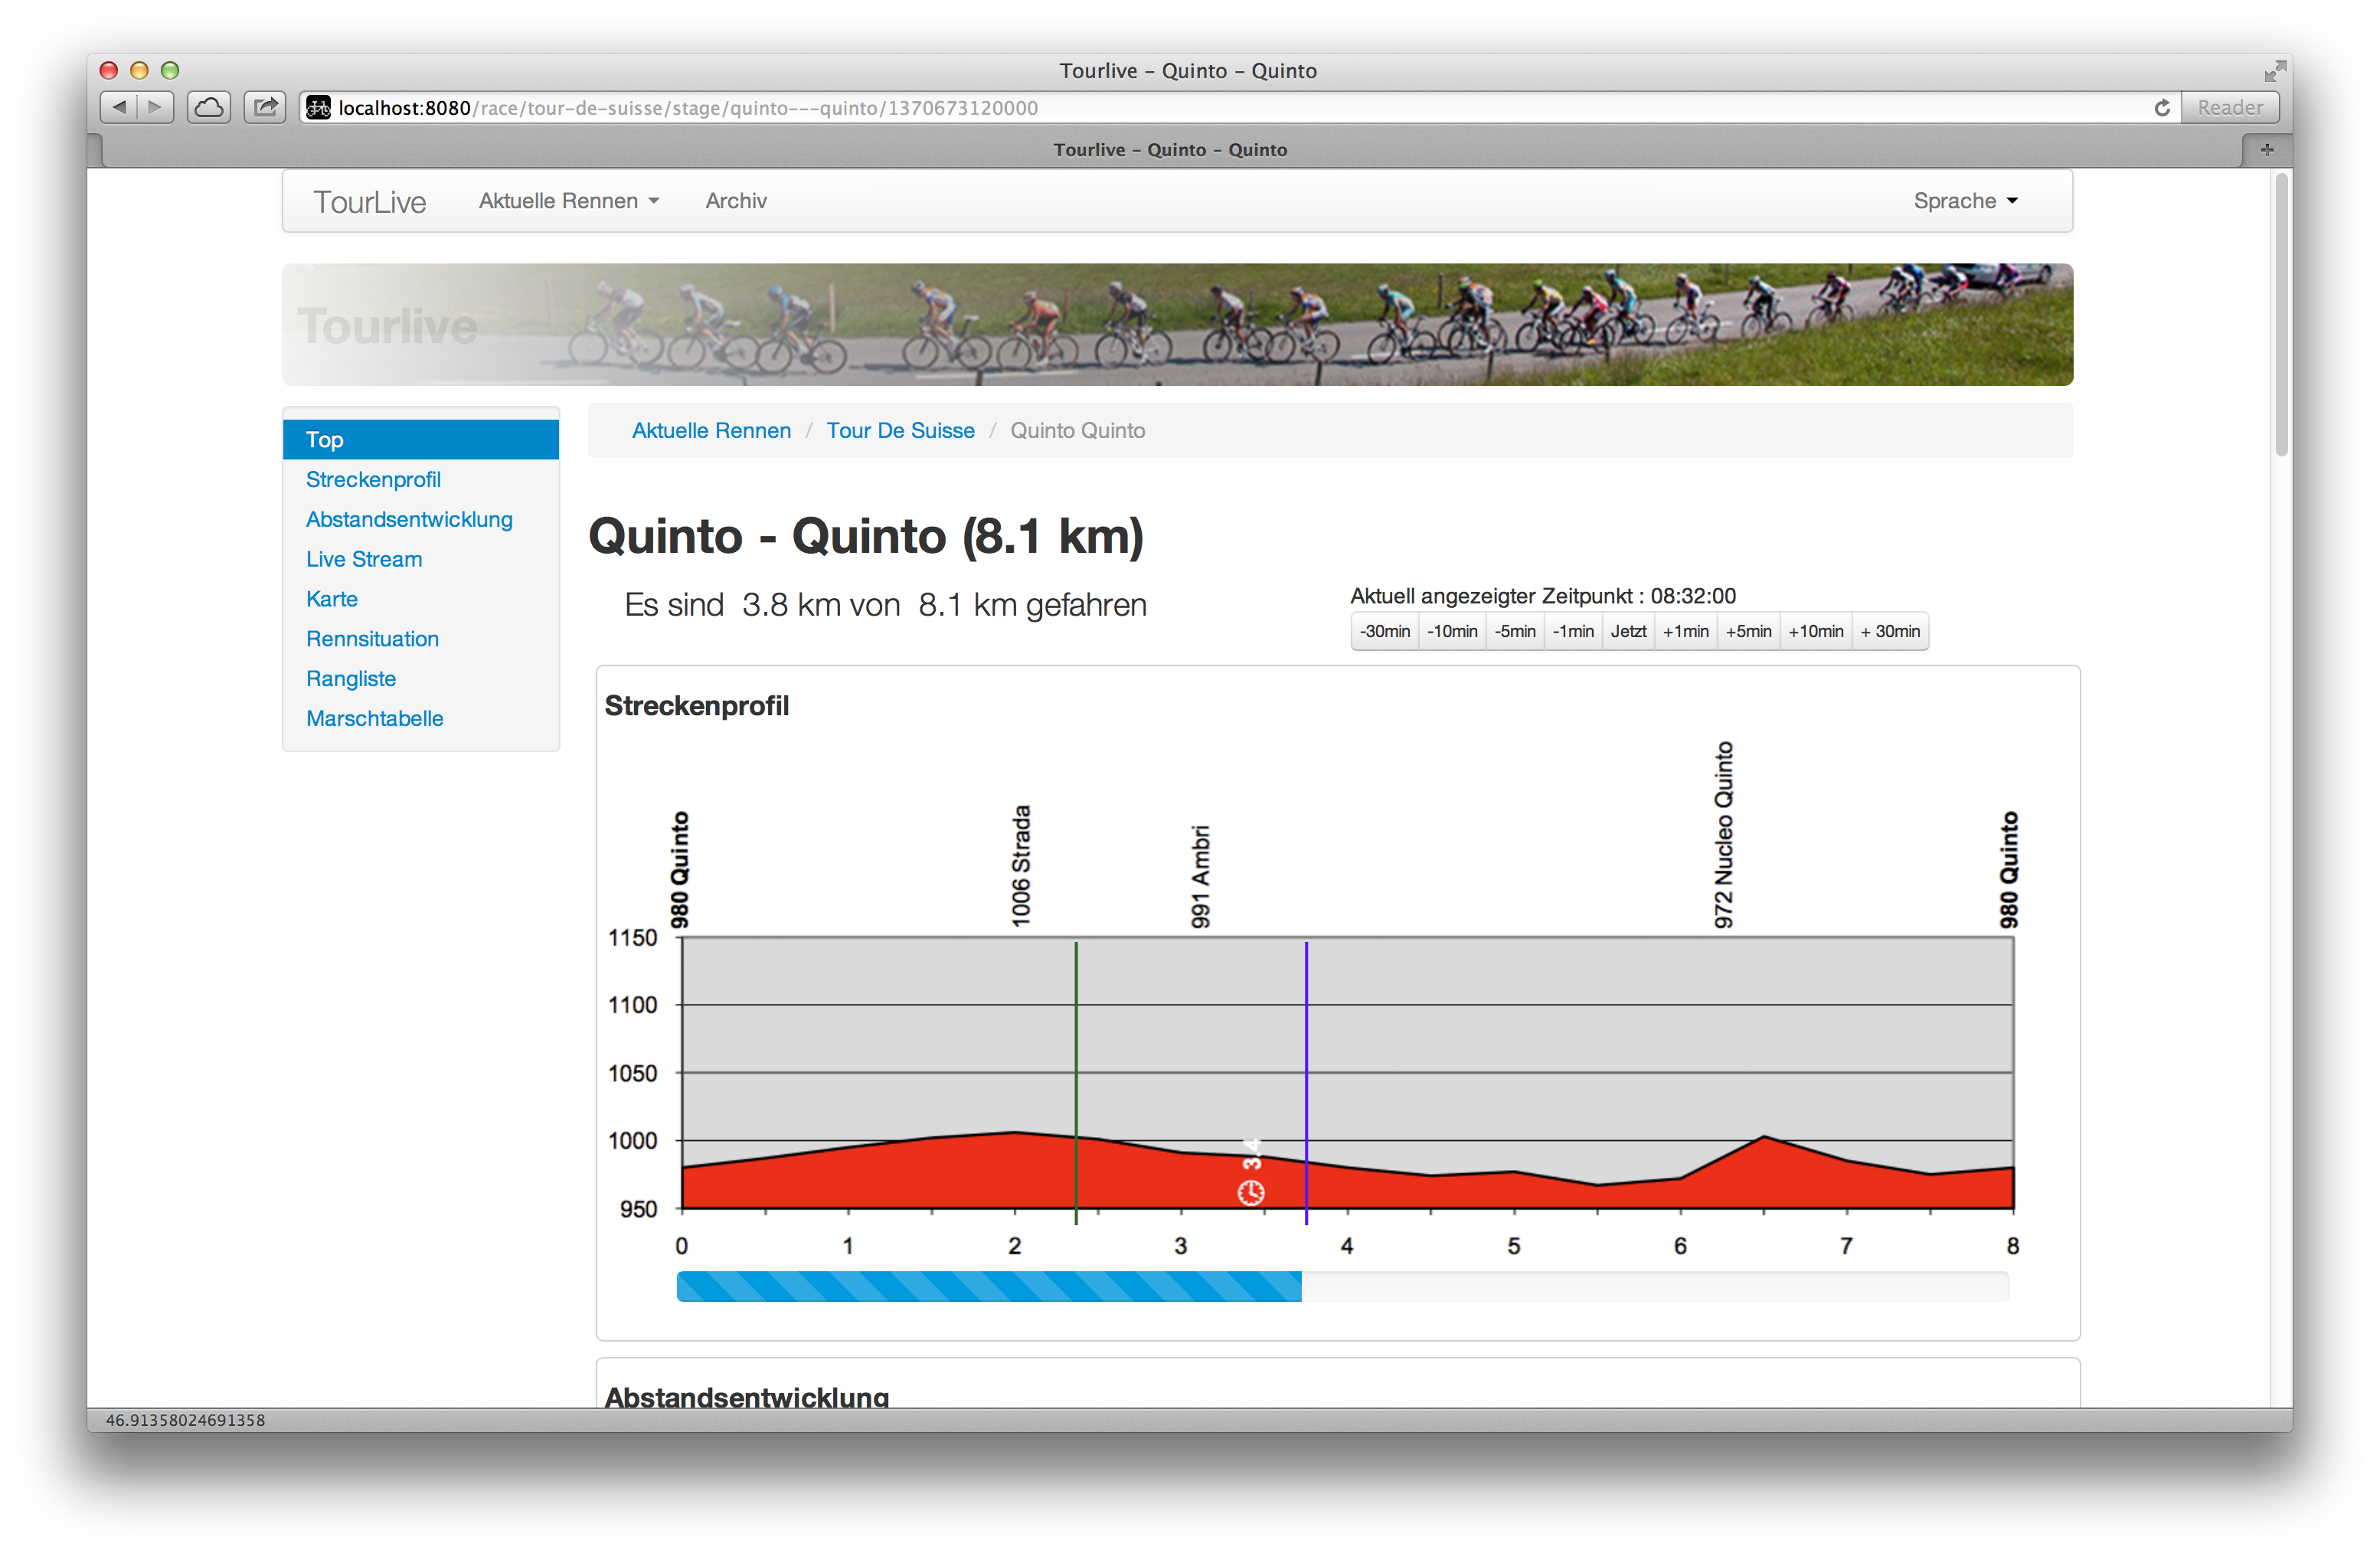
\includegraphics[width=130mm]{images/tourliveweb/tourlivewebansicht.png}
	\caption{TourLive Server Webseite anhand eines Beispiels}
	\label{fig:tourlivewebansicht}
\end{figure}

\subsection{Streckenprofil}
Die aktuelle Positionen der Aufnahmegeräte wird mittels eines HTML5 Canvas direkt auf das Etappenprofil gezeichnet. Dazu wird die JavaScript Library \textit{Raphaël JS}\footnote{Raphaël JavaScript Library, \url{http://raphaeljs.com/}, aufgerufen am 01.06.2013} verwendet. Zu jedem Gerät wird der aktuellste ValueContainer gesucht und daraus die Etappendistanz gelesen. Diese Distanz wird dann relativ zur Seitenbreite des Browserfensters als feine Linie mit der Farbe des Gerätes eingezeichnet wie in der Abbildung \ref{fig:tourlivewebansicht} zu sehen ist. Gleich unterhalb dieser Grafik befindet sich eine Statusanzeige [blau]. Sie zeigt die zurückgelegten Kilometer in dieser Etappe an und dient gleichzeitig auch als Navigation. Durch klicken an einer beliebigen Stelle im blauen Balken kann man zu dieser Stelle (Rennkilometer) im Rennen zurückspringen. Das Pendant zu dieser Navigation sind die Schaltflächen im oberen Bereich, welche das Rennen über die Zeit navigieren lassen.
\\

Gleich wie die Positionen der Aufnahmegeräte werden auch die Daten der Abstandsentwicklung mit der Raphaël JavaScript Library dargestellt.

